%                                                                 aa.dem
% AA vers. 9.1, LaTeX class for Astronomy & Astrophysics
% demonstration file
%                                                       (c) EDP Sciences
%-----------------------------------------------------------------------
%
%\documentclass[referee]{aa} % for a referee version
%\documentclass[onecolumn]{aa} % for a paper on 1 column  
%\documentclass[longauth]{aa} % for the long lists of affiliations 
%\documentclass[letter]{aa} % for the letters 
%\documentclass[bibyear]{aa} % if the references are not structured 
%                              according to the author-year natbib style

%
\documentclass{cosmo}  

%
\usepackage{graphicx}
%%%%%%%%%%%%%%%%%%%%%%%%%%%%%%%%%%%%%%%%
\usepackage{txfonts}
%%%%%%%%%%%%%%%%%%%%%%%%%%%%%%%%%%%%%%%%
%\usepackage[options]{hyperref}
% To add links in your PDF file, use the package "hyperref"
% with options according to your LaTeX or PDFLaTeX drivers.
%
\begin{document} 


   \title{Time-Delay Cosmography By H0LiCOW}

  \subtitle{New Precise $H_\mathrm{0}$ Measurements From Strong Gravitational Lensing System}

   \author{WeiLeong Tee
          \inst{1}
          }

   \institute{Department of Physics, University of Arizona, 
                1118 E. Fourth Street, Arizona\\
              \email{wltee@email.arizona.edu}
             }

   \date{Received November 26, 2020}

% \abstract{}{}{}{}{} 
% 5 {} token are mandatory
 
  \abstract{}{}{}{}{We review a new geometry method to measure Hubble constant $H_\mathrm{0}$ by using time-delay information in strong lensing systems by collaboration H0LiCOW/TDCOSMOS. This method is completely independent from other cosmic ladder approach, therefore act as a potential powerful tool to infer cosmological parameters and direct comparison with other results. High resolution images, long time light curves, lens galaxy velocity dispersion information are required for construction of lens model to predict time-delay distance $D_\mathrm{\Delta t}$, which is a direct probe to infer $H_\mathrm{0}$. Dominant systematic errors and solutions are briefly mentioned with no further implementation. In this work we modify the prior information on cosmological parameters and the functional form of $D_\mathrm{\Delta t}$ to observe the impact on original works. We derive 
  $H_\mathrm{0} = {{{73.50}}}_{{-1.82}}^{{+1.58}}\;\mathrm{km\,s^{-1}\,Mpc^{-1}}$, 
  consistent with H0LiCOW/TDCOSMOS works. The result can be improved in the future with inclusion of more strong lensing systems discovered by LSST.}
  
   \keywords{time-delay -- strong lensing -- Hubble constant -- H0LiCOW  --  cosmology 
               }

   \maketitle
%
%-------------------------------------------------------------------

\section{Introduction}

    Cosmological distance measurements have always been constantly investigated to constraint the nature of Universe. Starting from last century, the application of Hubble's Law 
    \begin{align*}
        c dt = a(t) \;dr \longrightarrow
    r = \int_0^z \frac{c dz}{H(z)}
    \end{align*}to describe the relationship between distance and Universe expansion has been extensively used to understand the expansion history. The current standard cosmological model, \emph{flat $\Lambda$CDM}, consisting of dark energy and cold dark matter in a spatially flat Universe has shown to best describe our observable Universe. With distance $D(r)$ and redshift $z$ measured, assume that Universe is matter and dark energy dominated, we can infer the cosmological parameters $H_\mathrm{0}, w$, curvature etc. by 
    \begin{align*}
        H^2 (z) = H_0^2 \left(\Omega_\mathrm{m} a^{-3}+\Omega_{\Lambda} e^{3 \int_{\log{a}}^0 (1+w)\;d\log{a}}+\Omega_\mathrm{k}a^{-2}\right)
    \end{align*}
    where $\Omega$ is density parameter and $a$ is scale factor. Recent Cosmic Microwave Background radiation (CMB) experiments, including the Wilkinson Microwave Anisotropy Probe (WMAP) and the Planck satellite and the Baryon Acoustic Oscillations (BAO) surveys, have provided stringent constraints with unprecedented precision on cosmological parameters within flat $\Lambda$CDM model.
    
    However, there have been discrepancies between different measurements about the Hubble constant ($H_{\rm{0}}$), cosmological parameter that quantify the expansion rate at local Universe as well as the age, size and critical density of the Universe. 
    There are two main categories in probing the local $H_{\rm{0}}$, luminosity and geometry probes. 
    The former luminosity method uses the standard candles, typically Type Ia supernovae, calibrated by Cepheid variable stars in local galaxies with precise period luminosity relation (P-L) to infer distance. Recent results from SH0ES program \citep{Riess2016} and Carnegie-Chicago Hubble Program \citep{Beaton2016} give $73.24 \pm 1.74 \;\mathrm{km\; s^{-1} \; {Mpc}^{-1}}$ and  $74.3 \pm 2.1 \;\mathrm{km\; s^{-1} \; {Mpc}^{-1}}$, respectively. 
    The latter measures the Baryon Acoustic Oscillations (BAO) in the galaxy clustering power spectrum, together with knowledge of sound horizon scale in understanding the fluctuations in the CMB, gives lower $H_\mathrm{0}$. Planck does not directly measure $H_{\rm{0}}$, but infer the value through sets of cosmological measurements by given assumptions on background cosmological model. From most recent Planck temperature data and Planck lensing under the flat $\Lambda$CDM model, $H_\mathrm{0}=67.8 \pm 0.9 \;\mathrm{km\; s^{-1} \; {Mpc}^{-1}}$; \cite{Abbott2018}, a combination work of clustering and weal lensing data, BAO and big bang nucleosynthesis gives $H_\mathrm{0}=67.4 \pm 1.1 \;\mathrm{km\; s^{-1} \; {Mpc}^{-1}}$; Some megamaser measurements also give similar results at lower value, although weaker significance in constraining the $H_\mathrm{0}$ boundaries.
    
    
    The current tension between so-called \emph{late Universe} and \emph{early Universe} results (Fig.\ref{fig14}) may result from unknown systematics or new physics that remain uncovered. Independent $H_\mathrm{0}$ measurement is crucial in examining other studies.
    There are degeneracy between $H_\mathrm{0}$ and other cosmological parameters in CMB analysis, for example if we slightly deviate from pure flat $\Lambda$CDM model, the inferred degenerate $H_\mathrm{0}$ value could be compatible with those higher values.Therefore a different measurement tool in getting $H_\mathrm{0}$ may help in breaking the degeneracy. 
    Another important reason for independent method is to minimize unavoidable, or even unknown systematic effects over surveys, such as metallicity dependence in the cosmic distance ladder, to verify the best underlying cosmological paradigm. With multiple independent datasets, all have roughly competitive precision in at least one parameter, we could constraint the cosmological parameters to unprecedented accuracy, and rule out the unwanted parameter spaces for future exploration.
    
    A new geometry method to $H_\mathrm{0}$ is through strong gravitational lensing with time-delays between multiple images. This has been shown to be completely independent approach from local distance ladder method, and able to constrain $H_\mathrm{0}$ up to $< 10 \%$ precision (e.g., \citealt{Suyu2010}, \citealt{Suyu2014}), and recently reach $\sim 2.4 \%$ from multiple lens systems \citep{Wong2019}. The strong lensing measurement is to measure the the deflected light from background source by foreground mass distribution that is located close along the line of sight, proposed by \cite{Refsdal1964}. When the background source is a variable source, such as active galactic nuclei (AGN) or a supernova, the variability is manifest in each of the multiple images, but existed time-delay in relative to each other due to the different light distorted paths. 
    
    This study has been inspired by the effort of collaboration H0LiCOW ($H_\mathrm{0}$ Lenses in COSMOGRAIL’s Wellspring, \citealt{Suyu2017}) lead by Suyu S. H., now in collaboration team Time-Delay Cosmography (TDCOSMOS). We give brief ideas of the original analysis, point out some of the dominant systematics, explain what has been modified and the subsequent results in the coming sections.
    
\section{Overview on Analysis}
    The time-delay, $\Delta t$, depends on the different light travelled paths, and therefore the time-delay distance $D_{\Delta t}$ and the lens mass distribution, 
    \begin{align*}
        \Delta t = \frac{D_{\Delta t}}{c} \Delta \phi_{\mathrm{AB}}
    \end{align*}
    where $\Delta \phi_{\mathrm{AB}}$ is the Fermat potential difference related to lens mass distribution, and $c$ is the speed of light. Fermat potential is defined as 
    \begin{align*}
        \phi (\theta, \beta) &\equiv \frac{\left(\theta - \beta\right)^2}{2}-\psi(\theta)\\
        \theta &: \text{image position}\\
        \beta &: \text{(unobservable) source position}\\
        \psi &: \text{lensing potential}
    \end{align*}
    Note that the commonly used deflection angle $\alpha$ and convergence (also named as surface mass density) $\kappa$ is defined through
    \begin{align*}
        \beta &= \theta - \alpha(\theta)\\
        \alpha (\theta) &= \nabla \psi (\theta)\\
        \kappa (\theta) &= \frac{1}{2} \nabla^2 \psi(\theta)
    \end{align*}
    The time-delay distance can be formulated as 
    \begin{align*}
        D_{\Delta t} \equiv (1+z_{\mathrm{d}})\frac{D_\mathrm{d} D_\mathrm{s}}{D_\mathrm{ds}}
    \end{align*}
    where $z_\mathrm{d}$ is the redshift of the foreground lens, $D_\mathrm{d}$ is the angular diameter distance to the lens, $D_\mathrm{s}$ is the angular diameter distance to the background source, $D_\mathrm{ds}$ is the angular diameter distance between the lenses and source. Because of the combination of angular distance measurements, $D_{\Delta t}$ is particularly sensitive to Hubble constant $(D_{\Delta t} \propto H_\mathrm{0}^{-1})$, and comparably less affected than others involving both local and non-local datasets upon calibration and analysis. 
    
    In practice, by measuring the time-delay from photometric light curves of the background source, one can determine the time-delay distance to the lens system and use the distance-redshift relation to infer $H_\mathrm{0}$. In order to accurately and precisely measure distance from foreground lenses, several information are needed regarding to the lenses and sources:
    (1) time-delays between multiple images, (2) high resolution and high signal to noise ratio images of the lens systems, (3) spectroscopic redshifts of the lens and sources, (4) lens mass model to determine the Fermat potential, (5) lens galaxy stellar velocity dispersion, this is particularly useful in determining the distance to the lens $D_\mathrm{d}$, (6) studies on lens environment. (5) and (6) are primarily served to break the lens model degeneracies.
    
     Fermat potential $\phi(\theta, \beta)$ depends strongly on both the mass distribution of the strong lens galaxy and the mass distribution of other galaxies along the line of sight. The source quasar properties need to be modeled simultaneously with the lens mass distribution to predict the observables. In particular, source position and intensity are needed to predict the positions, fluxes and time-delays of the lensed quasar images, whereas the source surface brightness distribution (of the quasar host galaxy) is needed to predict the lensed arcs. These observables, (1) image positions fluxes (2) time-delays (3) lensed arcs are then used to constrain the parameters of the lens mass model and the source.
    
    \begin{figure*}
        \centering
        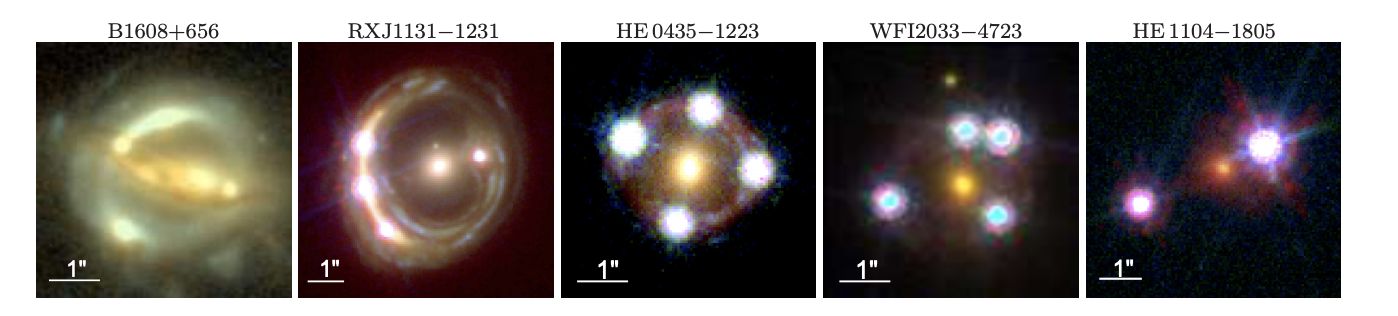
\includegraphics[width=\textwidth]{fig1_2.png}
        \caption{Lens images adopted from Fig.1 \cite{Suyu2017}. H0LiCOW lens sample, consisting of four quadruply lensed quasar systems in various configurations and one doubly lensed quasar system. The lens name is indicated above each panel.}
        \label{fig1}
    \end{figure*}
    
    \begin{figure}[h]
        \centering
        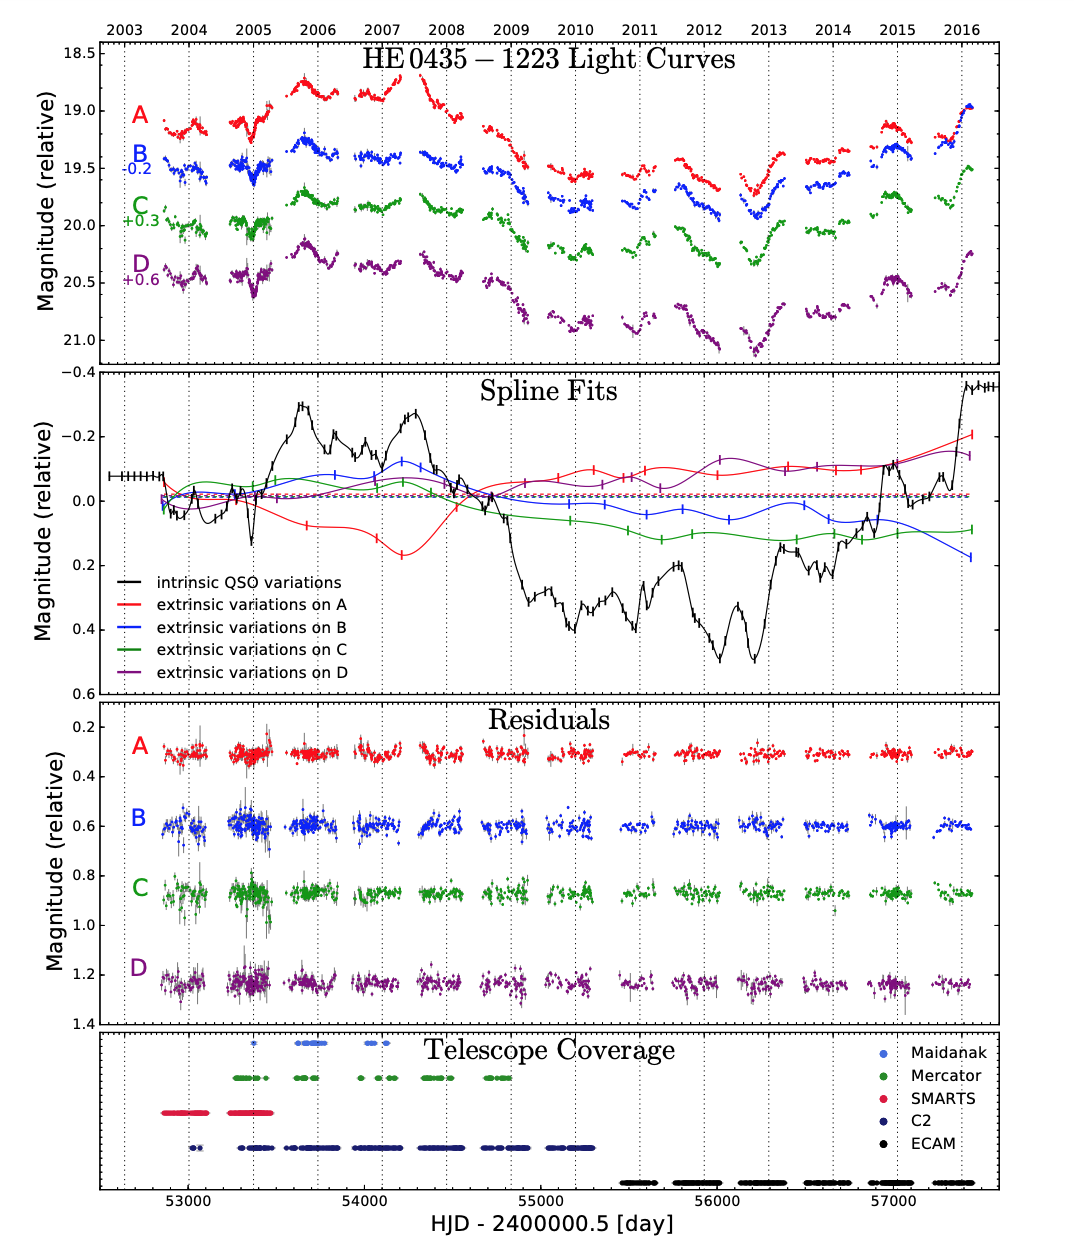
\includegraphics[width=0.48\textwidth]{fig2_2.png}
        \caption{Lens HE 0435-1223 light curves adopted from Fig.2 \cite{Bonvin2016}. From top to bottom: Light curves for the four lensed images of the quasar HE 0435-1223. The relative shifts in magnitude are chosen to ease visualization, and do not influence the time-delay measurements. The second panel shows a model of the intrinsic variations of the quasar (black) and the 4 curves for the extrinsic variations in each quasar image using the free-knot spline technique (color code). 
        The vertical ticks indicate the position of the spline knots. The residuals of the fits for each light curve is shown in the next panel. Finally, the bottom panel displays the journal of the observations for HE 0435-1223 for the 5 telescopes or cameras used to gather the data over 13 years, where each point represents one monitoring night.}
        \label{fig2}
    \end{figure}
    
    Fig.\ref{fig1} lists the current 5 time-delayed lens samples used in the H0LiCOW studies, and Fig.\ref{fig2} shows the light curve for lens HE0435-1223. These are all bright lensed quasars, being found in radio or optical quasar searches, monitored for around 13 years with 1 m class telescopes by the Cosmological Monitoring of Gravitational Lenses (COSMOGRAIL) team (now within TDCOSMOS). They have been followed up with high signal to noise Hubble Space Telescope ($\textit{HST}$) imaging and Keck spectroscopy for detailed modeling on lens mass system. 
    
    \begin{figure}[h]
        \centering
        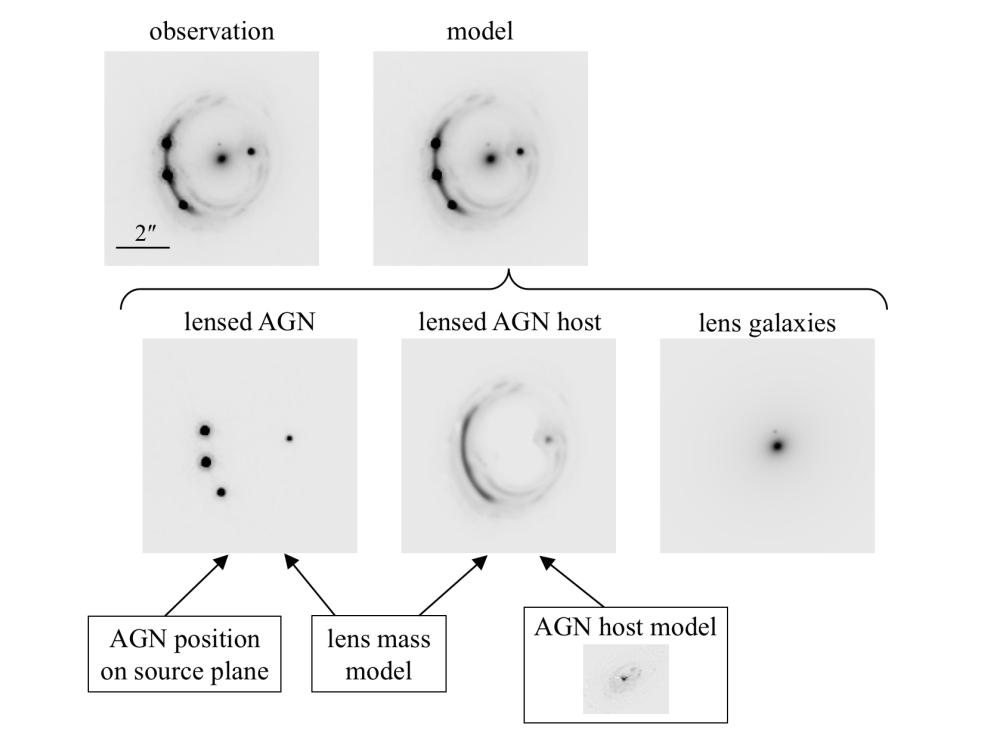
\includegraphics[width=0.48\textwidth]{fig3_2.png}
        \caption{Illustration of lens mass modelling of lens RXJ1131-1231, adopted from Fig.3  \cite{Suyu2018}. Top left is the observed \textit{HST} image. Top middle panel is the modeled surface brightness of the lens system, which is composed of three components shown in the second row: lensed AGN images (left), lensed AGN host galaxy (middle), and foreground lens galaxies (right). The bottom row shows that a mass model is required together with the AGN source position and AGN host galaxy surface brightness, to model the lensed AGN and lensed AGN host images.}
        \label{fig3}
    \end{figure}
    
    Wide field spectroscopy and multiband imaging of lens environment have been obtained for all lens samples, especially detail structure along the line of sight. Furthermore, the lens galaxy spectroscopy for lens stellar velocity dispersion has also be measured and serve as tool to overcome the lens mass modelling degeneracy addressed below. Fig.\ref{fig3} shows the construction of lens mass model using full information from surface brightness distribution.
    
    To obtain $D_{\Delta t}$ information, accurate lens modeling on lens mass distribution is essential to predict the time-delays. Given modelled background source surface brightness $I(\beta)$, the image surface brightness $I(\theta(\beta))$ being distorted by the lens can be predicted and compare with observation. Specifically, the likelihood we compute is 
    \begin{align*}
        \log P(\theta|I_\mathrm{obs}) \sim \chi^2 \left( \frac{I(\theta)-I(\theta)_{\mathrm{obs}}}{2}\right) + S(I(\beta)) 
    \end{align*}
    Deep, high resolution $\textit{HST}$ imaging with image residual levels consistent with noise allows the full extraction on image intensities and Einstein Rings structure. With additional information on background point source position, together with knowledge in lens mass model and source host galaxy model, model construction of lensed source and lensed source host galaxy that produced the arcs and ring structures is plausible and the results are being compared with observation. See Fig.\ref{fig3} for illustration.
    
    One of the problem in modelling the lens mass distribution is the strong degeneracy between radial mass profile slope of lens and $D_{\Delta t}$ (see \citealt{Suyu2012} for detail). Because time-delays primarily depends on the average surface mass density between multiple images, time-delays can also used to constrain the radial mass profile slope. An increase in time-delays $\Delta t$ with same lens galaxy surface mass density can be either result from a larger $D_{\Delta t}$ and hence smaller $H_\mathrm{0}$ or a slower decline in the lens galaxy radial profile. The intrinsic scatter in radial mass profile slope has also damaged the precision to infer cosmological parameters. It is important to have high accuracy and precision measurements on the radial profile slope of the lens galaxy near the lensed images of the quasars, therefore require more observation studies on the lens system.
    
    Once a model of the convergence (surface mass density, $\kappa$) is constructed, from lens theory it states that the following family of models $\kappa_{\lambda}$ fits equally well to the observed lensing data,
    \begin{align*}
        \kappa_{\lambda} = \lambda + (1-\lambda)\kappa
    \end{align*}
    where $\lambda$ is a constant. This transformation is analogous to adding a constant mass sheet $\lambda$ in convergence, and rescaling with $1-\lambda$ to keep same mass within the Einstein radius, it is therefore called the \emph{mass-sheet degeneracy}. Such transformation corresponds to a rescaling of the background source coordinate by a factor $1-\lambda$, preserve the observed image morphology and brightness invariant.
    The Fermat potential and time-delays transform as 
    \begin{align*}
        \phi_{\lambda} (\theta, \beta) &= (1-\lambda) \phi(\theta, \beta) + f(\beta)\\
        \Delta t (\theta) &= (1-\lambda) \Delta t (\theta) 
    \end{align*}
    and thus impact time-delay distance $D_{\Delta t}$ which uses to infer $H_\mathrm{0}$. For example, the lens has shifted toward observer with same surface brightness, with same time-delays $\Delta t$, $D_{\mathrm{\Delta t}}$ appears to be larger and therefore concludes with incorrect smaller $H_\mathrm{0}$. Fig.\ref{fig4} explained how mass-sheet degeneracy would affect the arrival times and convergence given three different convergence distributions.  
    
    \begin{figure}[h]
        \centering
        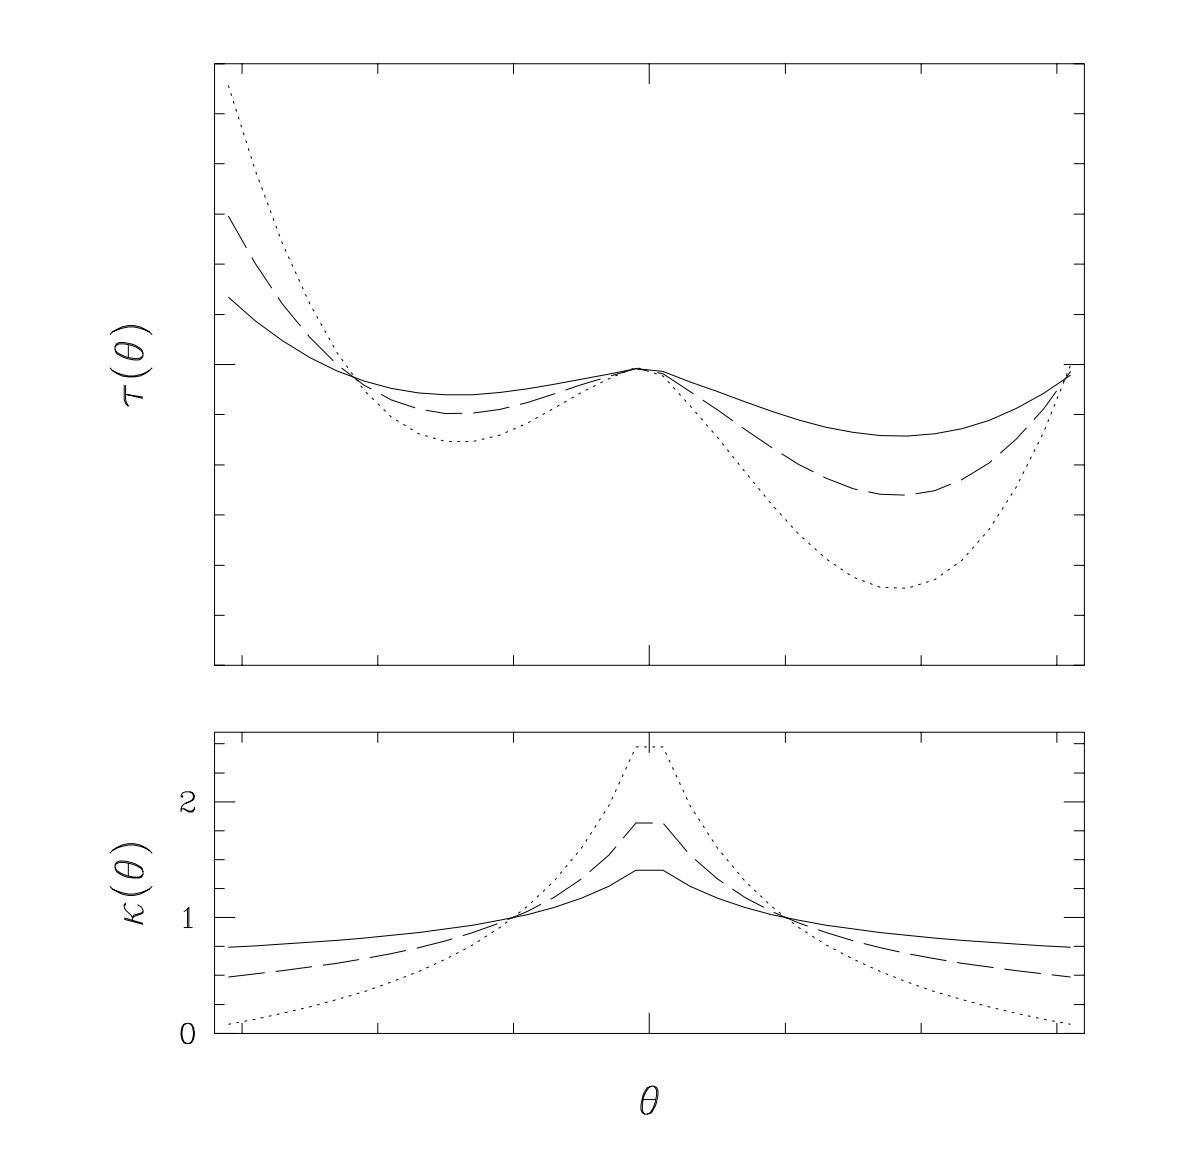
\includegraphics[width=0.48\textwidth]{fig4_2.png}
        \caption{Mass-sheet degeneracy explained in Fig.12 of \cite{Courbin2002}. Illustration of the mass disk degeneracy, showing the surface density (lower panel) and the arrival time (upper panel) for three circular lenses. The arrival time indicates a saddle point (which looks like a local minimum in this cut), a maximum, and a minimum. The dashed curves correspond to a non-singular isothermal lens. Stretching the time scale amounts to making lens profile steeper (dotted curves) and shrinking the time scale amounts to making the lens profile shallower (solid curves).}
        \label{fig4}
    \end{figure}
    
    To break the mass sheet degeneracy, high resolution lens environment data and lens galaxy velocity dispersion and stellar kinematics are necessary. \emph{External convergence}, $\kappa_\mathrm{ext}$ is defined as the external convergence factor that caused by mass structure(typically galaxy densities) in local and along the light of sight to the lensing system. $\kappa_\mathrm{ext}$ distribution can be measured from N-body simulation by matching the slightlines to observed overdensity in galaxy densities. With $\kappa_\mathrm{ext}$ the true time-delay distance can be calculated via the form:
    \begin{align*}
       D_\mathrm{\Delta t} = \frac{D^{\mathrm{model}}_\mathrm{\Delta t}}{1-\kappa_\mathrm{ext}}
    \end{align*}
    where $D^{\mathrm{model}}_\mathrm{\Delta t}$ is the time-delay distance derived from lens modeling. These collective datasets are used in the likelihood analysis, with prior knowledge on $P(\kappa_\mathrm{ext})$ to marginalized cosmological parameters. Fig.\ref{fig5} work explained the inclusion of stellar kinematics in lens galaxy helps breaking the degeneracy.
    \begin{figure}[h]
        \centering
        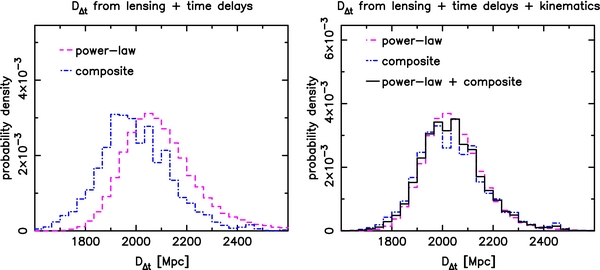
\includegraphics[width=0.48\textwidth]{fig5_2.png}
        \caption{Illustration on how lens velocity dispersion information breaks the mass-sheet degeneracy from Fig4. \cite{Suyu2014}. Time-delay distance, $D_{\Delta t}$, for the power-law model (dashed) and the composite model of baryons and dark matter (dot-dashed). The left panel is based on only the lensing and time-delay data, whereas the right panel includes the information from the lens velocity dispersion. The stellar kinematic information on the lens galaxy helps break lens model degeneracies, yielding very similar $D_{\Delta t}$ distributions for the two lens models. The combined PDF of $D_{\Delta t}$ is shown in solid in the right panel.}
        \label{fig5}
    \end{figure}
    Moreover, stellar kinematics and velocity dispersion of strong lens galaxy provides an independent mass measurement within the effective radius to complement the lensing mass enclosed within the Einstein radius. With kinematic information on the lens galaxy, we can determine the angular diameter distance to the
    lens, $D_\mathrm{d}$, independent of $\kappa_\mathrm{ext}$. Information from $D_\mathrm{d}$ helps breaking degeneracies
    among cosmological parameters, particularly for models beyond flat $\Lambda$CDM.
    
    For cosmological parameters inference, the analysis makes use of multiple datasets. We denote the observation datasets as $\left\{ \boldsymbol{d_\mathrm{HST}, \Delta t, \sigma, d_\mathrm{LOS}} \right\}$, where $\boldsymbol{d_\mathrm{HST}}$ is the \textit{HST} (and AO, if available) imaging data, $\boldsymbol{\Delta t}$ for the time-delays, $\boldsymbol{\sigma}$ for the velocity dispersion of the lens galaxy, and $\boldsymbol{d_\mathrm{LOS}}$ for the properties of the LOS mass distribution determined from photometric and spectroscopic data. For joint Bayesian likelihood analysis, the parameter sets are defined as:
    \begin{align*}
        \boldsymbol{\pi} &= \{H_\mathrm{0}, \Omega_\mathrm{m}, \Omega_\mathrm{\Lambda}, \Omega_\mathrm{k}, w \} \\
        \boldsymbol{\xi} &= \{\boldsymbol{\pi}, \boldsymbol{\nu}\}
    \end{align*}
    where $\boldsymbol{\pi}$ is cosmological parameters set, $\boldsymbol{\nu}$ represents lens model parameters and nuisance parameters including the $\kappa_\mathrm{ext}$ and other parameters that either contribute to the systematic errors or to break model degeneracy. We also define $\boldsymbol{A}$, as a discrete set of assumptions make about the model form, data modeling, set-up, and treatment. We want to obtain the posterior probability distribution function (PDF) of the model parameters $\boldsymbol{\pi}$ given the data, $P(\xi|d_\mathrm{HST}, \Delta t, \sigma, d_\mathrm{LOS}, A)$ by marginalized over the nuisance parameters $\boldsymbol{\nu}$, 
    \begin{align*}
        P(\pi\,|\,d_\mathrm{HST}, \Delta t, \sigma, d_\mathrm{LOS}, A) = \int d\nu\;P(\xi\,|\,d_\mathrm{HST}, \Delta t, \sigma, d_\mathrm{LOS}, A)
    \end{align*}
    For likelihood analysis, 
    \begin{align*}
        P(\xi\,|\,d_\mathrm{HST}, \Delta t, \sigma, d_\mathrm{LOS}, A) \propto P(d_\mathrm{HST}, \Delta t, \sigma, d_\mathrm{LOS}\,|\,\xi, A)P(\xi\,|\,A) 
    \end{align*}
    where $P(\xi\,|\,A)$ contains the priors information given assumptions. Since the datasets are independent, the likelihood can be separated,
    \begin{align*}
        P(d_\mathrm{HST}, \Delta t, \sigma, d_\mathrm{LOS}|\xi, A) = & P(d_\mathrm{HST}|\xi, A) \times P(\Delta t|\xi, A)\\ 
        & \times P(\sigma|\xi, A) \times P(d_\mathrm{LOS}|\xi, A)
    \end{align*}
    Individual likelihoods are calculated separately and combine with priors PDF to get the final posterior PDF for a given set of assumptions. 
    
    Blinding is one of the key concept in modern analysis to avoid cognitive bias toward preferable result. Blind likelihood analysis in getting distances, $D_{\Delta t}$ and $D_\mathrm{d}$ has been adopted to avoid choosing values that shift toward expected result. In the intermediate steps when multiple lens models producing $D_{\Delta t} \,(D_\mathrm{d})$, median value of $D_{\Delta t}\,(D_\mathrm{d})$ is subtracted from and only the distribution is used for output. Note that various commonly used source and lens models have been considered and used in distance calculation, the average $D_{\Delta t}\,(D_\mathrm{d})$ distribution is used for the final cosmological parameter inference. After the analysis has been completed and all committee members agree, the median value would be add upon the result to obtain the true $H_\mathrm{0}$. Fig.\ref{fig6} shows one of the intermediate $D_\mathrm{\Delta t}$ calculated with and without blinding process, the unblinding is obtained after the analysis is done to reveal the true distance. 
    \begin{figure}[h]
        \centering
        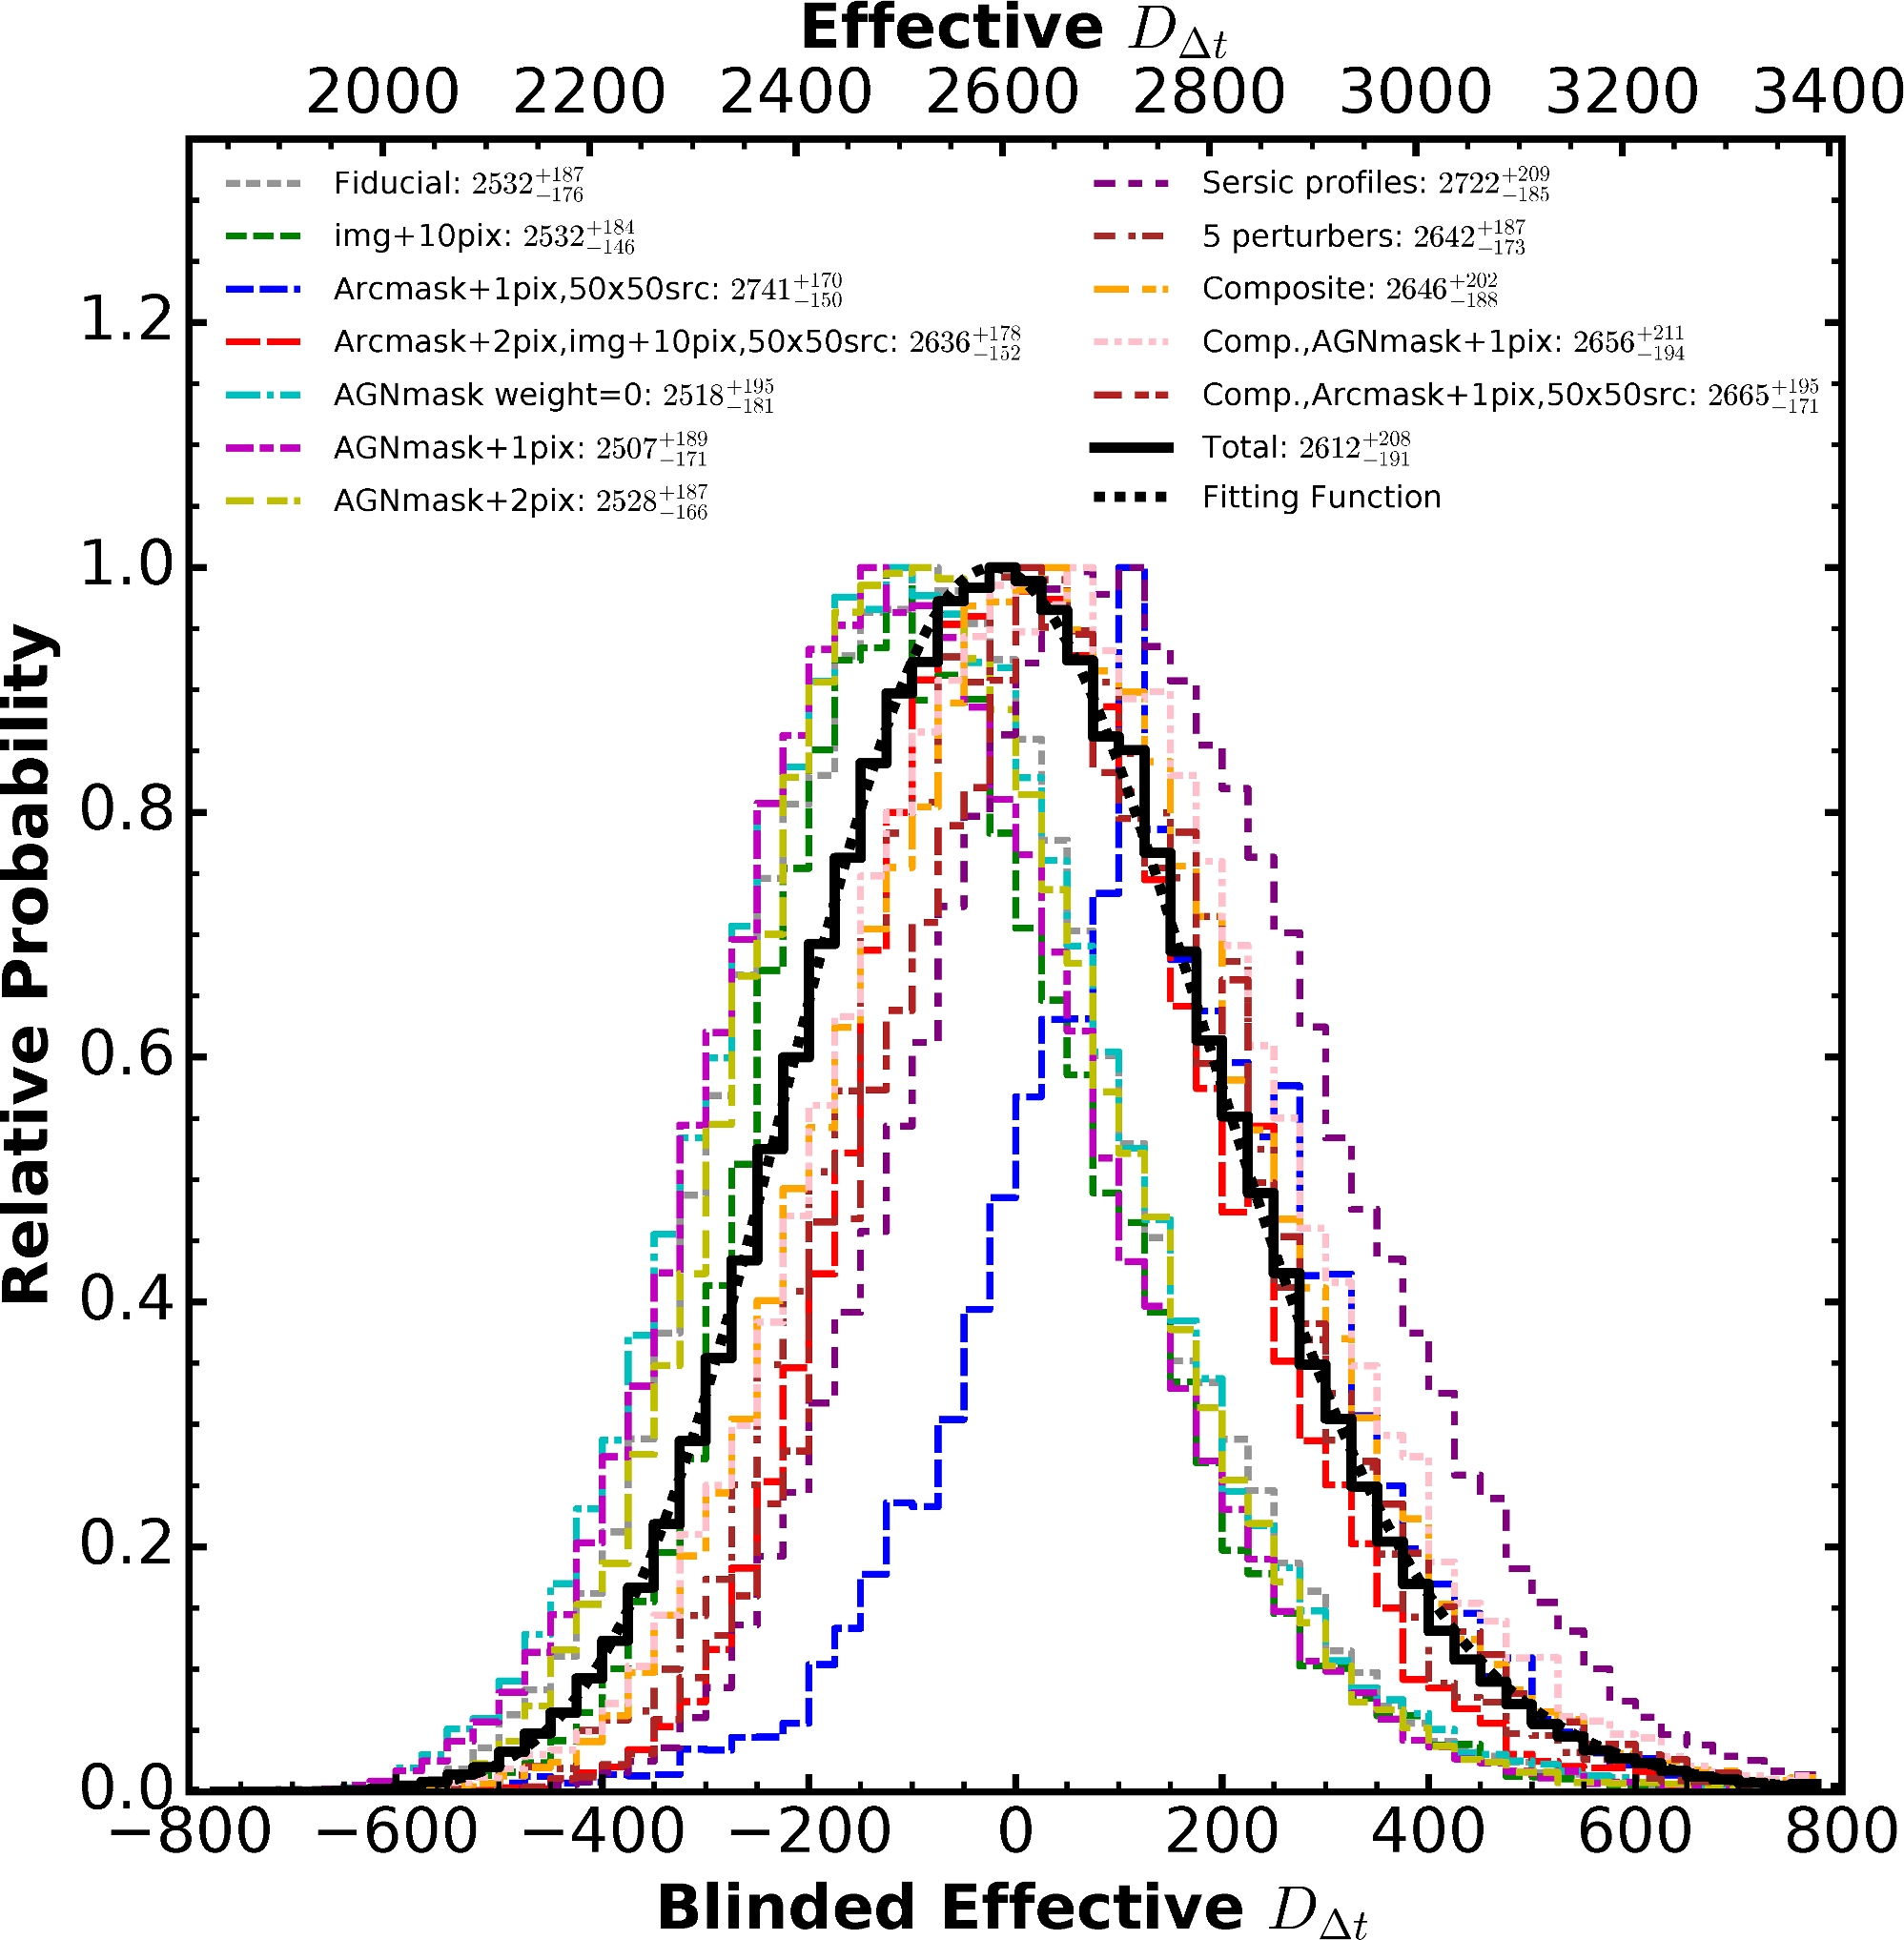
\includegraphics[width=0.48\textwidth]{fig6_2.png}
        \caption{PDF of $D_{\Delta t}$ for the various models, from Fig.8 in \cite{Wong2016}. The median and 68 $\%$ quantile of each distribution is given. The thick black line represents the sum of all the distributions, which accounts for the various systematic uncertainties. The dotted black line is the skewed lognormal distribution fit to the final distribution. The bottom x-axis shows the blinded result, which is obtained by subtracting the median of the combined PDF from the absolute $D_{\Delta t}$ values. The top x-axis shows the true $D_{\Delta t}$ values. Throughout blind analysis, the top x-axis was hidden until analysis was finalized.}
        \label{fig6}
    \end{figure}

\section{Modification and Results of Joint Likelihood Analysis}
    The cosmological models considered in this work are flat-$\Lambda$CDM (FLCDM), open-$\Lambda$CDM (oCDM), flat-CDM with Equation of State parameter $w$ (F$w\,$CDM), CDM with time-varying $w$ which parametrized as $w(z)=w_\mathrm{0} + w_\mathrm{a}\;z/(1+z)$ ($w_\mathrm{0} w_\mathrm{a}$CDM). We adopt a simplified version of original likelihood analysis. We deploy 30 walkers and 20000 chains in the Markov Chain Monte Carlo (MCMC) Sampler by using Python package \textit{emcee} for a rather smooth sampling result. With given $D_\mathrm{\Delta t}$ and $D_\mathrm{d}$ distributions from marginalized observed datasets and lens modelling, to obtain posterior PDF of cosmological parameters, only two variables are allowed to tune: (1) functional form of $D_\mathrm{\Delta t}$ for $H_\mathrm{0}$ inference, (2) priors of the cosmological parameter sets. In original works a skewed lognormal function fit has been applied to the posterior distributions on $D_\mathrm{\Delta t}$ to derive $H_\mathrm{0}$. 
    
    We adopt three different distributions for $D_\mathrm{\Delta t}$, (1) a normal distribution, (2) a skewed lognormal distribution with narrower width, (3) kernel density estimation (KDE) given observed $D_\mathrm{\Delta t}$. The first method gives the worst result and can only serve as testing purpose, the other two methods return similar result. We prefer KDE estimation because it makes no assumption on the functional form of distance PDF, only derive cosmological parameters from the data alone, although requiring data input complicates and lengthens the computation time.
    
    In H0LiCOW works, cosmological parameters $\boldsymbol{\pi}$ have flat priors. In their results, time-delay distances give stringent constraint on $H_\mathrm{0}$ but only weakly constraint other parameters, as shown in Fig.9 \cite{Wong2016}. At the beginning, we only change the $H_\mathrm{0}$ prior to a normal distribution PDF and all the others remain flat distribution,
    \begin{align*}
        P(H_\mathrm{0}) \sim \mathcal{N} (70,30)
    \end{align*}
    The result as shown in Fig.\ref{fig7}, $\Omega_\mathrm{m}$ has a rather broad scatter for tight $H_\mathrm{0}$ values.
    \begin{figure}[h]
        \centering
        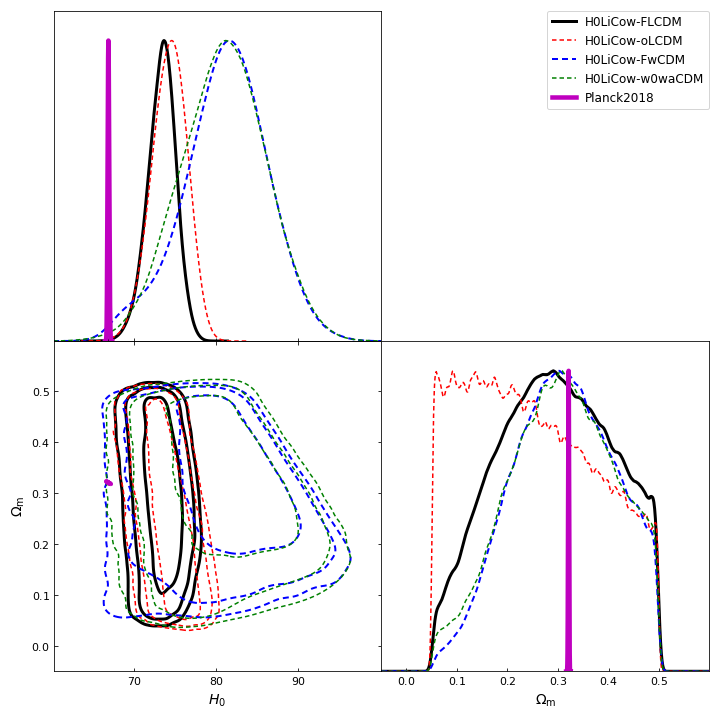
\includegraphics[width=0.48\textwidth]{H0LiCOW-Planck-H0N.png}
        \caption{$P(H_\mathrm{0}) \sim \mathcal{N}(70,30)$ and other parameters are flat priors.}
        \label{fig7}
    \end{figure}
    Since we already have prior knowledge on other cosmological parameters, we decide to adopt normal distribution on all priors, as listed in Table \ref{table1}, for our main results. We derive the Hubble constant to be 
    \begin{align*}
        H_\mathrm{0} = {{{73.50}}}_{{-1.82}}^{{+1.58}} \;\; \mathrm{km}\mathrm{s}^{-1}\mathrm{Mpc}^{-1}
    \end{align*}

\begin{table*}
\centering
\begin{tabular}{|c|c|c|c|c|c|}
\hline
Cosmological models & $H_\mathrm{0}$  & $\Omega_\mathrm{m}$ 
& $\Omega_\mathrm{k}$     & $w\,/\,w_\mathrm{0}$      
& $w_\mathrm{a}$ \\ \hline
FLCDM       & $\mathcal{N}(70,30)$ & $\mathcal{N}(0.3,0.1)$ 
& -     & -      
& -      \\ \hline
oLCDM       & $\mathcal{N}(70,30)$ & $\mathcal{N}(0.3,0.1)$ 
& 
\begin{tabular}[c]{@{}c@{}}
$\mathcal{N}(0,0.2)$\\  $(1-\Omega_\mathrm{m}-\Omega_\mathrm{k}>0)$
\end{tabular} 
& -         & -      \\ \hline
F$w\,$CDM        & $\mathcal{N}(70,30)$ & $\mathcal{N}(0.3,0.1)$ 
& -   & $\mathcal{N}(-1.5,1)$ 
& -      \\ \hline
$w_\mathrm{0}w_\mathrm{a}\,$CDM   & $\mathcal{N}(70,30)$ & $\mathcal{N}(0.3,0.1)$ 
& -    & $\mathcal{N}(-1.5,1)$ 
& $\mathcal{N}(0,1)$ \\ \hline
\end{tabular}
\label{table1}
\caption{Prior PDF entering likelihood analysis.}
\end{table*}

    \begin{figure}[h]
        \centering
        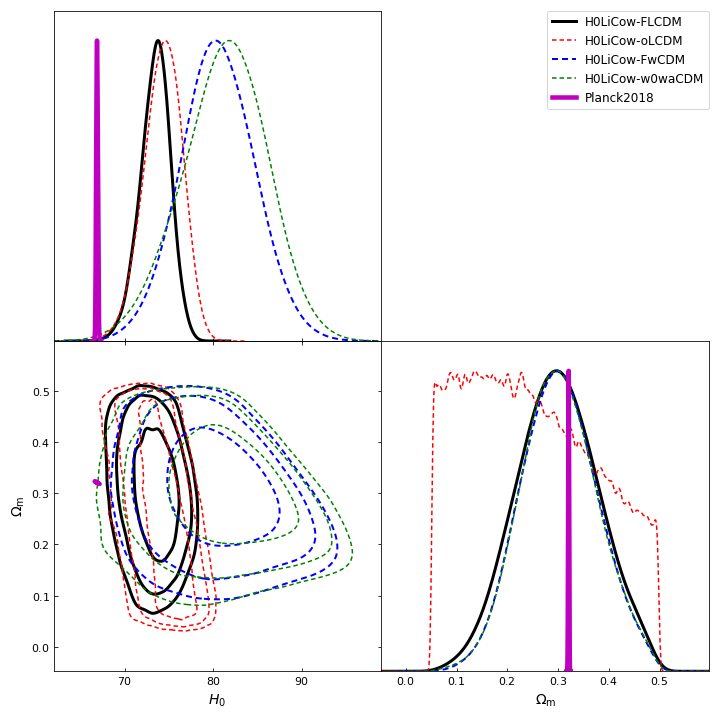
\includegraphics[width=0.48\textwidth]{H0LiCOW-Planck-allN.png}
        \caption{All priors are normal distributed.}
        \label{fig8}
    \end{figure}
    Comparing Fig.\ref{fig7} and Fig.\ref{fig8}, there are no significant distinction, and $\Omega_\mathrm{m}$ has biased toward the prior functional form in the latter scenario. We also show the MCMC result of Planck2018 data by using Python package \textit{cobaya}. Planck2018 has strongly peaked at smaller $H_\mathrm{0}$ value, which is in obvious contrast with this work. 
    
    \begin{figure}[h]
        \centering
        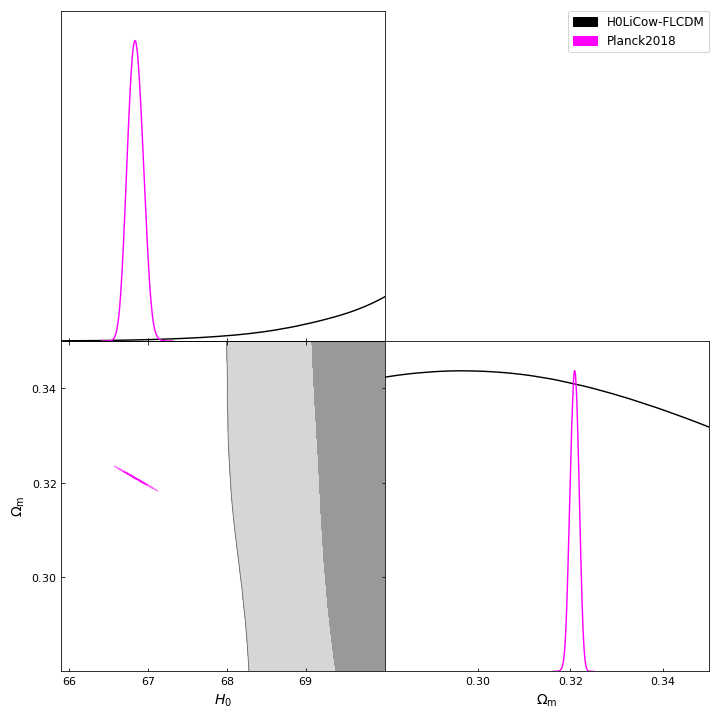
\includegraphics[width=0.48\textwidth]{H0LiCOW-Planck-allN-zoom.png}
        \caption{Zoom in to show the the significant difference
        between Planck2018 and this work.}
        \label{fig9}
    \end{figure}
    
    We also show the posterior PDF for all cosmological model parameters in Fig.\ref{fig10}-Fig.\ref{fig13}.
    
    \begin{figure}[h]
        \centering
        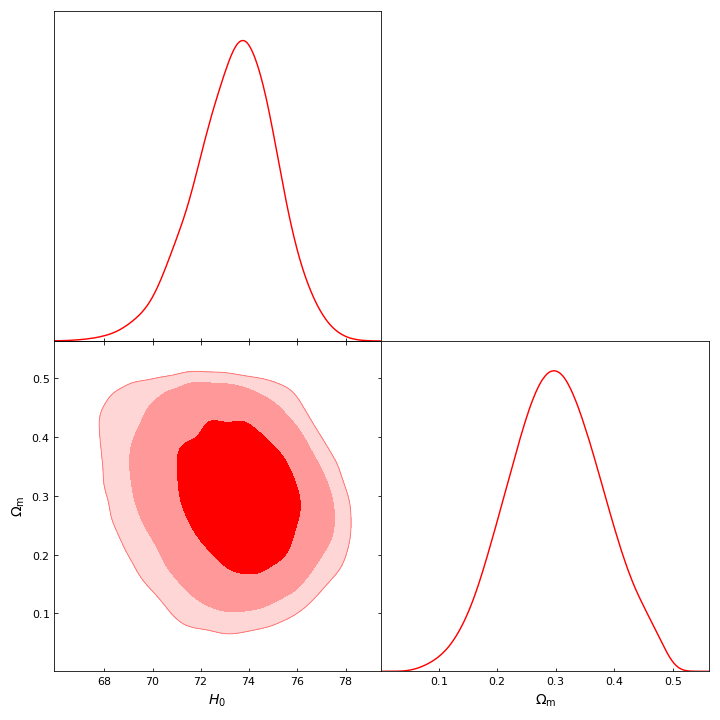
\includegraphics[width=0.4\textwidth]{H0LiCOW-FLCDM-allN.png}
        \caption{FLCDM}
        \label{fig10}
    \end{figure}
    \begin{figure*}[h]
        \centering
        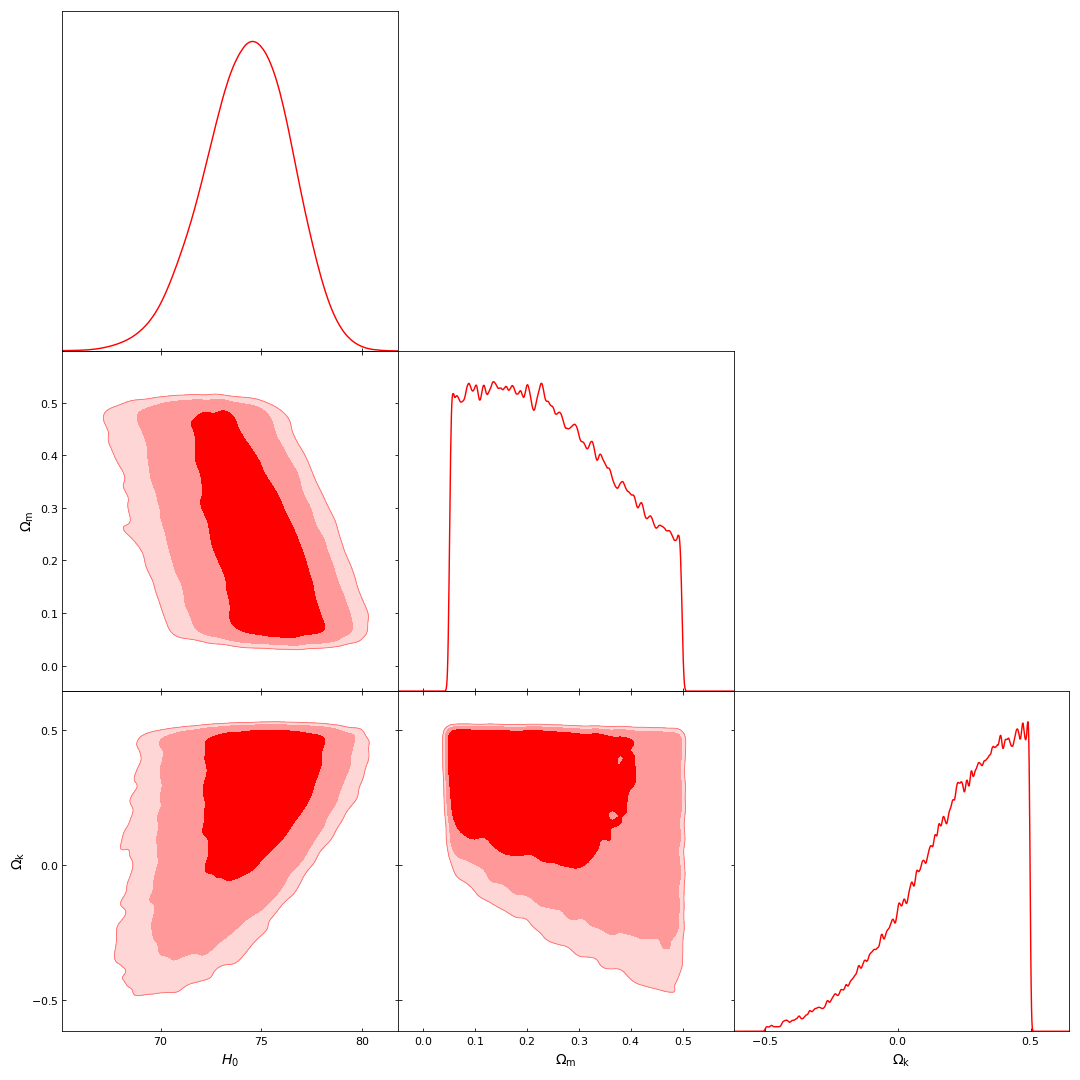
\includegraphics[width=0.7\textwidth]{H0LiCOW-oLCDM-allN.png}
        \caption{oLCDM}
        \label{fig11}
    \end{figure*}
    \begin{figure*}[h]
        \centering
        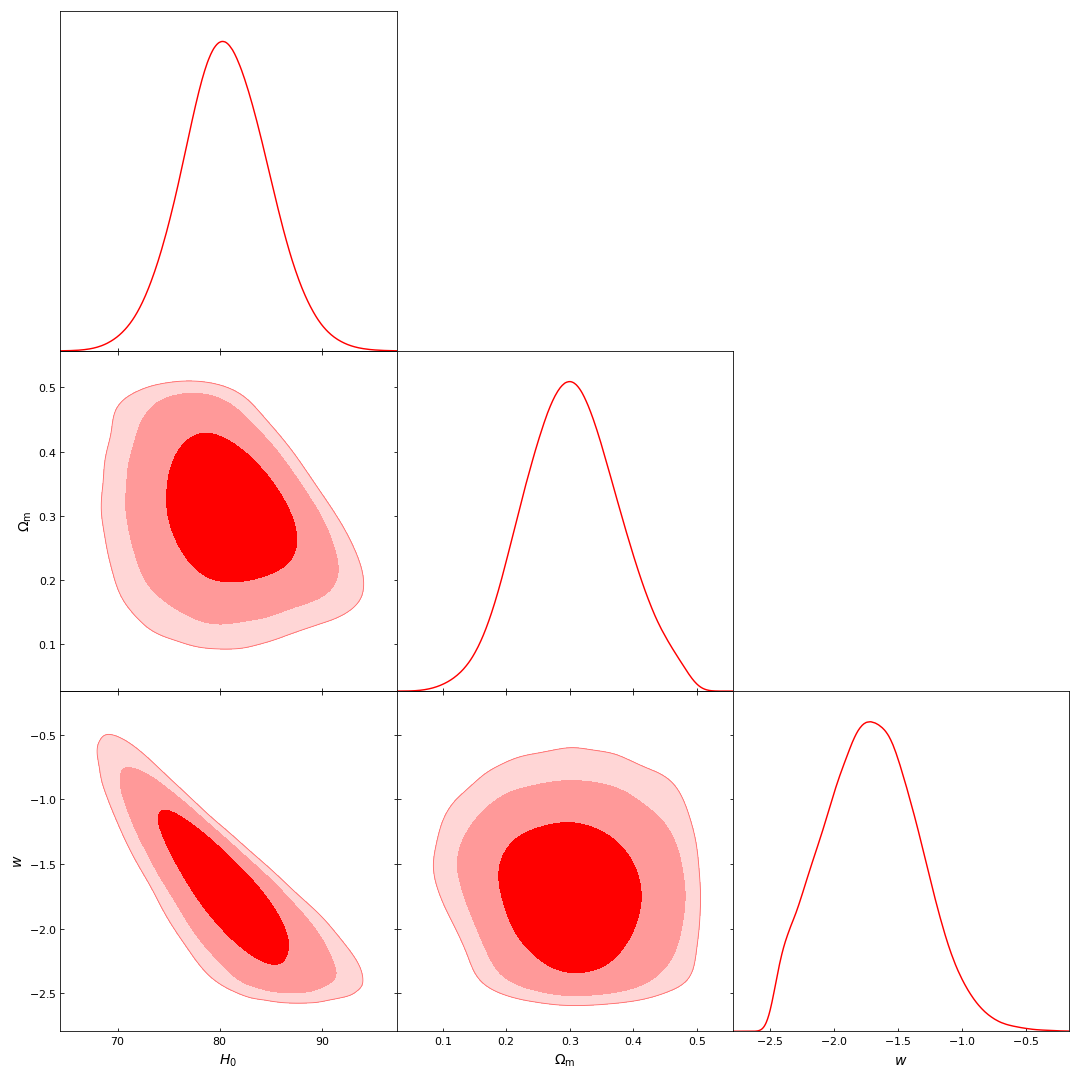
\includegraphics[width=0.7\textwidth]{H0LiCOW-FwCDM-allN.png}
        \caption{F$w\,$CDM}
        \label{fig12}
    \end{figure*}
    \begin{figure*}[h]
        \centering
        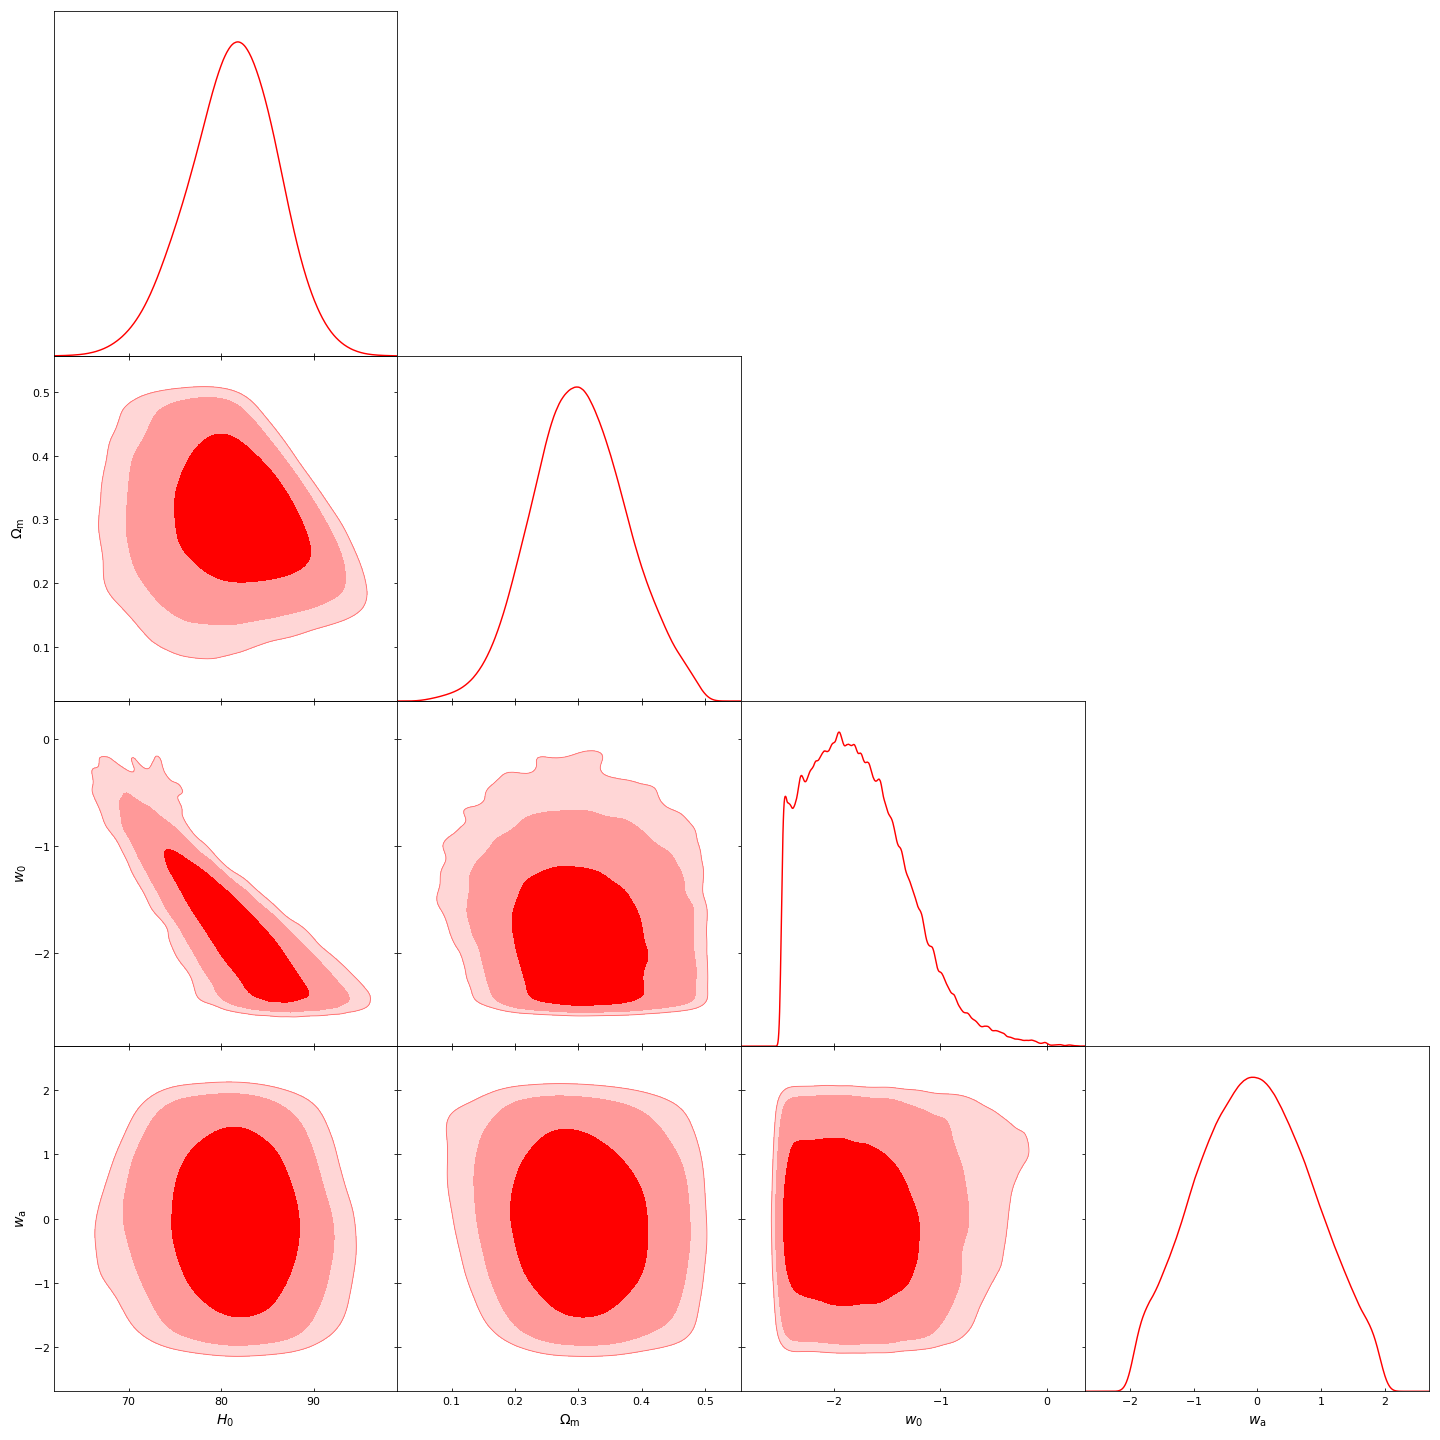
\includegraphics[width=1\textwidth]{H0LiCOW-w0waCDM-allN.png}
        \caption{$w_\mathrm{0}w_\mathrm{a}\,$CDM}
        \label{fig13}
    \end{figure*}
    
\section{Conclusion}
\begin{figure*}[h]
        \centering
        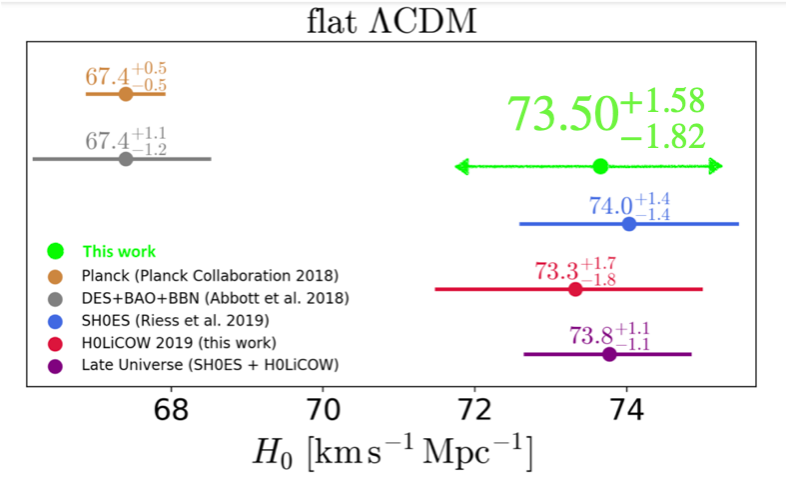
\includegraphics[width=1\textwidth]{fig20_2.png}
        \caption{$H_\mathrm{0}$ tension plot from Figure 12 in \cite{Wong2019}, together with this work.}
        \label{fig14}
\end{figure*}
time-delay cosmography is a completely independent method to infer cosmological parameters. The simple picture on using gravitational lens time-delays to measure $H_\mathrm{0}$ has proven to be successful. The advantages in getting rid of propagated systematics in calibration of cosmic ladder has greatly improved the reliability and accuracy of this work. Observation datasets on high resolution light curves, imaging, lens LOS studies, lens galaxy velocity dispersion are essential ingredients for not only reconstruction of lens mass model but also into solving parameter degeneracies. Blind analysis has been adopted to make sure cognitive bias does not lead the analysis into preferable direction. With only few strong lens systems with joint likelihood analysis, we are able to constraint Hubble constant down to within $3 \%$, the results are expected to improve in the future when more lens systems discovered by Rubin Observatory within the 10-year Legacy Survey of Space and Time (LSST). 

\begin{acknowledgement}
This work mainly follows the presentation
given by Phil Marshall in 2017 SLAC Summer Institute \citep{Matshall2017}.
Special thanks to Geoff Chih-Fan Chen (postdoc in UCLA,
H0LiCOW/TDCOSMOS) on helping with the concept building process.
\end{acknowledgement}

% WARNING
%-------------------------------------------------------------------
% Please note that we have included the references to the file aa.dem in
% order to compile it, but we ask you to:
%
% - use BibTeX with the regular commands:
\bibliographystyle{aa} % style aa.bst
\bibliography{WL_cosmology} % your references Yourfile.bib
%
% - join the .bib files when you upload your source files
%-------------------------------------------------------------------


\end{document}
